%\documentclass[10pt,a4paper,final,oneside,openany,article]{memoir}
%\documentclass[letterpaper,a4paper,10pt]{article}
\documentclass[10pt,letterpaper,final]{article}
\usepackage[utf8]{inputenc}
\usepackage[british]{babel}
\usepackage{hyperref}
\setcounter{tocdepth}{3}
\usepackage[draft]{fixme}
\usepackage{abstract}
\usepackage{todonotes}

%% FONT
%\usepackage[T1]{fontenc}
%\usepackage{lmodern}
%\usepackage[urw-garamond]{mathdesign}
% Fonts configuration
%  - Palatino and Bitstream Vera Sans Mono for verbatim
\usepackage[T1]{fontenc}
\usepackage{palatino}
\usepackage[sc]{mathpazo} % Math font for Palatino
\usepackage{bera}
\linespread{1.05} % Palatino needs more leading (space between lines)
\usepackage{microtype}
\usepackage{graphicx} % ++
\usepackage{color}
\definecolor{kugrey}{rgb}{.4,.4,.4}
\usepackage{listings}
\lstset{ %
    language=Python,                % choose the language of the code
    frame=single,                   % adds a frame around the code
    keywordstyle = \footnotesize\ttfamily,
    commentstyle = \color{kugrey}\textit,
    stringstyle = \ttfamily,
    basicstyle   = \footnotesize\ttfamily,
    numberstyle=\tiny,
    sensitive = true,
}

%% odds and ends
%\chapterstyle{hangnum}
\setcounter{secnumdepth}{2}

%HEADINGS
\title{Constructing Models For Diagnosing Rare Diseases\\
        \small{by Using the Google Search Engine}}

\author{Brian S. Mathiasen $-$ soborg@diku.dk \\
        Henrik G. Jensen $-$ henne@diku.dk\\
%        \\
%        Department of Computer Science\\
%        University of Copenhagen\\
%        Universitetsparken 1\\
%        DK-2100 Copenhagen, Denmark
}

\date{\today} %\today

%%
\begin{document}
\maketitle
\listoffixmes
%\tableofcontents


\begin{abstract}
In this paper we design and construct models for assisting physicians
with the task of diagnosing rare diseases. Using a prior knowledge of
rare diseases consisting of \textit{disease name, some symptoms} and
\textit{synonyms}, we utilize the \textit{Google Search Engine} to build
the model over several iterations. The model is constructed using
machine learning and natural language processing techniques by text
mining symptoms and features from abstracts and other interesting
paragraphs of text found in the search process.
\todo[inline]{Tests and results}

\end{abstract}
%%-----------------------------
%\newpage

\section{Preface}
\subsection{Expectations to the reader}
The reader is expected to have knowledge in Computer Science at a
Master's degree level.

It is expected that the reader has read the project
\cite{jensenandersen}, which explains the foundations needed for this
project.

We expect the reader to have knowledge of Natural Language Processing
techniques, in particular POS-tagging and phrase chunking.


\section{Introduction}
\label{chap:introduction}
Physicians have expressed a need for aiding in the process of diagnosing
rare diseases \cite{googlingdiagnosis}, and point towards using the
Internet as a resource for information gathering, with particular focus
on utilizing Google or other popular search engines
\cite{googlechangemedicine} \cite{diagnosissearchengines}.

%The current process of automating this process relies heavily on static
%information, which is only expanded through manual interaction. \fxwarning{citation needed}
%\url{http://www.wrongdiagnosis.com/},
%\url{http://www.rarediseases.org/}, \url{http://www.orpha.net/}.

In this project, we investigate methods for automating information
collection of specific features from rare diseases, with focus on
establishing a model with which a practising physician may query a case
report for some patient and get a prediction of possible diseases based
on the knowledge of the model.
To increase the prediction precision, we must expand the model and look
into harvesting specific information of some disease through a number of
iterations on popular search engines. We use Natural Language Processing
(NLP) provided through a Python library \cite{NLTK} to extract unique
information from some description of the disease, and use Machine
Learning to refine the search within the model.

%by assuming certain semantic and
%syntactic properties of symptoms and medically related phrases and
%terms.

In the following we will present and highlight current and previous work
within this domain. In chapter 3, we will discuss our method
methodically, with particular focus on construction of model and feature
extraction and post processing of harvested information.
Then we will explain how we tested the system and argue statistical
significances by comparing to previous work, as well as assessing the
viability of our system as it is.
Finally we will conclude our paper and discuss implications and other
thoughts relevant to our method, while also proposing a number of topics
for future work.

\subsection{Limitations}
\todo[inline]{Blanks to be filled.}

\section{Previous Work}
Current work by Radu Dragusin and Paula Petku investigate the same
thesis of automating information gathering as those we are presenting.
However, as this is a work in progress we do not have access to further
information at this point in time \cite{radupaula}.

\cite{jensenandersen} proposed a system for diagnosing rare diseases
using vector space models and text mining. They showed a potential in
automating such a process, but their results were not statistically
significant. Their system did not rely on prior knowledge of particular
diseases, but still showed that around 60\% of the tests were
satisfactory.


The article \cite{googlingdiagnosis} proves the viability of using
Google as a diagnosis aid, despite the tests being done manually with
little consideration with regard to automation or test reliability and
validity.

%Our system will move on to the next step and introduce intelligent
%automation through a number of predefined criteria and utilizing several
%machine learning and natural language processing techniques.


%The editorials \cite{googlechangemedicine} and
%\cite{diagnosissearchengines} suggest Google and search engines in
%general as being a very strong player in the task To perform the initial
%testing we mimicked the previous project where a TF-IDF\footnote{Term Frequence - Inverse Document Frequence.} matrix was build
%using information (abstracts,titles, keywords) gathered form Pubmed. The
%knowledge of search engines being a valuable source of information is
%apparent, but the shear amount of misinformation and noise from regular
%searches make such a method in it’s current incarnation unreliable and
%error prone.\fxwarning{citation needed} \todo[inline]{Omformuler,
%præciser!}


%(Our goal is to refine and provide means for filtering out this noise
%and focus on harvesting information from related material with reference
%to the original search terms as well as specific criteria for the text
%mining process.)


%Inspiration for a system: Online Search Engine specialised for
%diagnosing stuff etc.
%http://www.healthline.com/symptomsearch

%This system is based on simple searches that relies on an already
%established database of diseases with appropriate meta-information. The
%user is able to search for symptoms and can narrow down the search by
%adding several symptoms. The system will then present a list of possible
%diseases according to some relevance criterion.

%(It is an end-user focused system, while our system will be a back-bone
%focused system, attempting to establish a model on which queries may be
%imposed. It will as such automate the information collection based on
%several machine learning and natural language processing techniques
%appropriate for the needs.)


%Google Health: http://www.google.com/intl/en-US/health/about/index.html


%Article by practising doctor on “do’s and don’t’s when using Google as
%diagnosis aid”:
%http://vitualis.wordpress.com/2007/02/26/google-based-medicine/


\section{Method}
Data received from Orphanet, an online database of information
specialised on rare diseases, is initially used as prior knowledge to
harvest additional information from the Internet.



As one of the premises of the project was to introduce prior knowledge
of the disease model, we needed to process our available data. We were
given a large corpus of data from Orphanet \ref{app:orphanet},
consisting of \texttt{\{orphanum, disease name, disease
description/abstract, maybe author and date\}} for each disease in the
data set.\todo[inline]{Rewrite this nonsense.}


The data is processes similar to the method described in
\cite{jensenandersen}, and will thus be used too bootstrap our knowledge
of each disease, allowing us to iterate and harvest additional
information using various harvesting techniques roughly covering the use
of the \textit{Google} search engine to collect an array of websites
given a query relevant to the disease (disease name and a possibly a
number of keywords). For each website, we will collect paragraphs and
save it for further processing if the cosine angle between the two
vectors is within a reasonable threshold. For each accepted paragraph we
use NLP to identify candidates for relevant terms and phrases that will
then be used to expand the model. The abstract flow model is available
in figure \ref{fig:flow}.


\begin{figure}[htp!]
\begin{center}
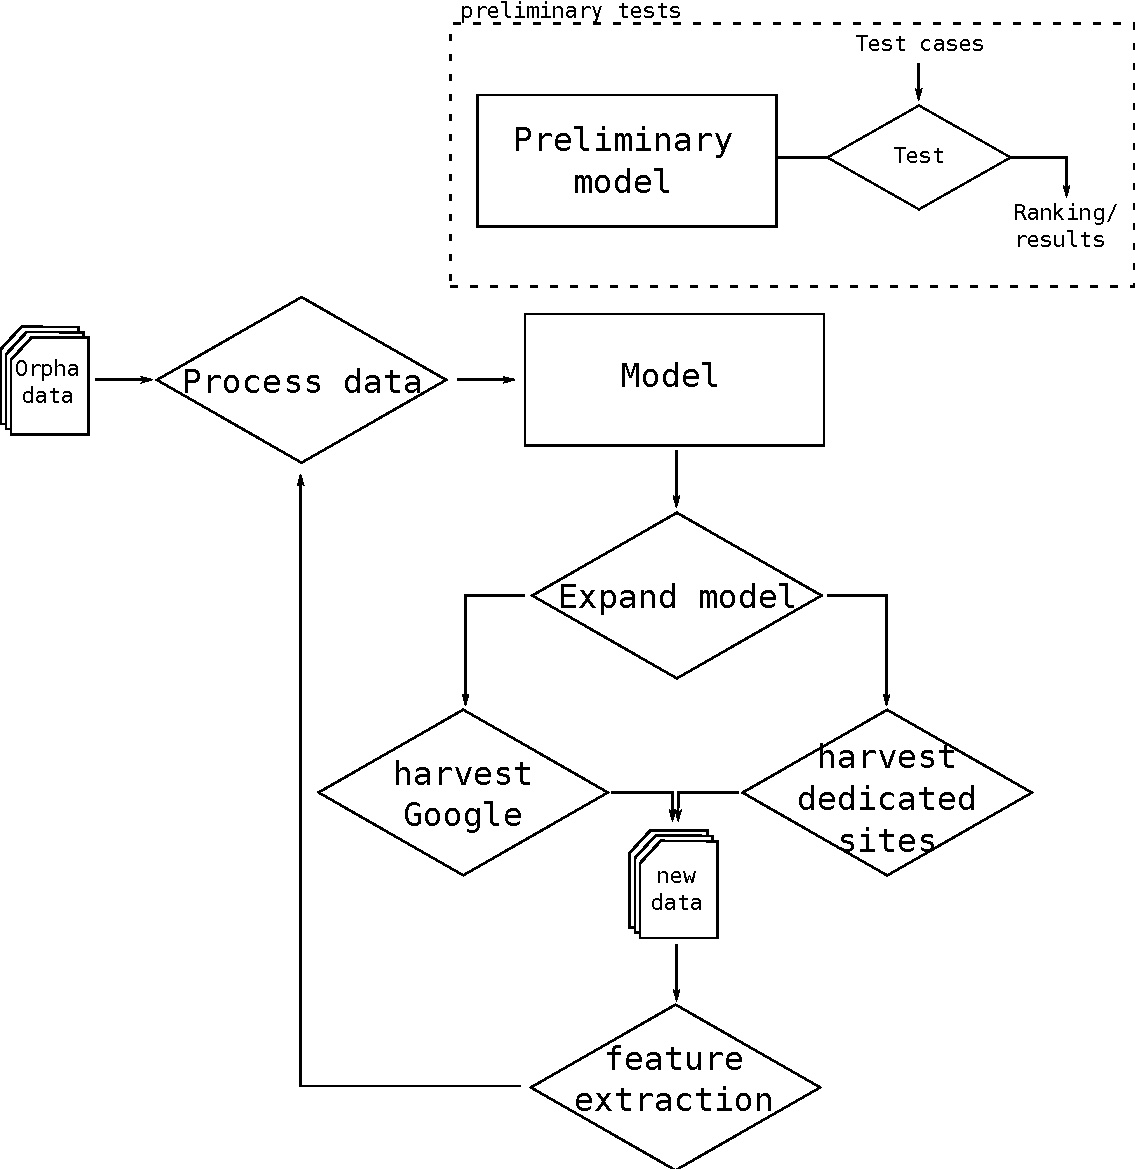
\includegraphics[scale=0.4]{images/pipeline}
\caption{Systems diagram}
\label{fig:flow}
\end{center}
\end{figure}

The process will be described in greater detail in the following
sections.

\todo[inline]{Something N-gram machine learning here.}

\subsection{Building the preliminary model}
To perform the initial testing we mimicked the setup of
\cite{jensenandersen} where a TF-IDF matrix was build using information
(abstracts,titles, keywords) gathered form Pubmed.

A sparse term-disease matrix (similar to the well-known term-document
model) was build over the abstracts received from Orphanet. Each row in
the matrix thus represented a feature vector of a disease with the
features being a list of term frequencies. Prior to the creation of the
matrix, the terms were stemmed (using the Porter stemming algorithm) and
stopwords\footnote{The stopwords are a list of 127 English words provided
by the Python NLTK library
(\texttt{nltk.corpus.stopwords.words("english")}} were removed along
with non-alphanumerical\footnote{Symbols not represented in the Danish
Alphabet} symbols. The term-disease matrix were then processed using the
TF-IDF model (as originally proposed by \cite{tfidf}) along with
additional logarithmic smoothing of the $tf_{t,d}$-parameter to flatten
term-burstiness (\cite{burstiness}). The TF-IDF model
\[
w_{t,d} = log(tf_{t,d}+1)\cdot log\frac{|D|}{|\{d'\in D|t\in d'\}|}
\]
where $tf_{t,d}$ is term frequency of term $t$ in disease $d$, $|D|$ 
the total number of diseases in the disease set, and $|\{d'\in D|t\in
d'\}|$ the number of diseases containing the term $t$.

To compare the precision of the new model to the previous, we made the
same queries to the model using the same scoring-scheme to obtain a rank
for each disease. The rank of each disease represents the precision of
the model.

A query is given, stemmed and stopwords are removed. Each
disease-vector that contain one or more of the queried terms is given a
score which is based on a summation of each of the weights of the
queried terms relevant to the disease.
\[
s_{d} = \displaystyle\sum\limits_{t_1}^{t_n} w_{t,d}\quad t \in Q
\]
\todo[inline]{write a more reasonable formula}
Though the model used in \cite{jensenandersen} was based on large
amounts of information gathered from PubMed, our tests showed that we
could obtain close to the same precision solely based on the abstracts
from Orphanet. This indicates large amounts of noise in previous project
where the information (or model) of each disease was based on
non-validated abstracts from PubMed using customised queries. The
results can be seen in appendix \ref{app:preliminary_results}.


\subsection{Harvesting data}
Harvesting additional data to expand our existing TF-IDF model is done
using the Google search engine. For each site corresponding to our
query, disease name and a number of keywords from disease abstract, we
extract paragraphs and measure the relevance of that paragraph compared
to the corresponding abstract from Orphanet. The comparison is measured
using a cosine covariance measure of two term vectors representing
known information, $\textbf{s}$ and a harvested paragraph of information
$\textbf{p}$
\[
similarity(\textbf{s}, \textbf{p}) = \frac{\textbf{s} \cdot \textbf{p}}{||\textbf{s}|| ||\textbf{p}||}
\]
Which, using formula provided by the NLTK library gives us a score
between $0$ and $1$, where 0 is complete correlation and 1 is no
correlation. The acceptance threshold for paragraphs collected for
further processing is set to $0.8$. This number is used based on a
number of anecdotal tests showing a reasonable amount of relevant
information, where $0.9$ would introduce too much noise, and $0.7$
being too strict.
\todo[inline]{Write pseudocode for this harvesting and paragraph
selection procedure}


%The comparison consists of constructing a $2 x n$ matrix, for $n$ being
%the number of unique terms in both texts, after which the cosine
%similarity measure is calculated and accepted paragraphs pushed onto
%further processing.

\subsection{Feature Extraction}
Feature extraction is used as a means to extract unique or otherwise
relevant information from a document regarding a specific disease. It
consists mainly of POS-tagging and subsequent chunking into phrases,
involving a nested iteration through an array of POS-taggers and
subsequent chunking by exploiting certain syntactic and semantic
properties of sentences.


The POS-tagging procedure, also referred to as a
braubt \cite{} \footnote{Brill, Regexp, Affix, Unigram, Bigram, Trigram}
tagger is built using the following strategies, in decreasing order of
complexity and context exploitation:
\begin{description}
\item[Unigram tagging] A unigram tagger finds the most likely tag for each word
in the training corpus and uses that information to assign tags to new
tokens.
\item[Bigram tagging] A bigram tagger work similarly to the unigram
tagger, except it finds the most likely tag for each word given the
preceding tag.
\item[Trigram tagger] This tagger works like the bigram tagger, except it
uses two pieces of information. N-gram taggers assigned tags to tokens
depending on the $N - 1$ preceding tags.
\item[Affix tagging] The affix tagger is similar to the unigram tagger.
It takes some fixed-size substring of a word and finds the most likely
tag for that substring.
\item[Regexp tagging] This tagger assigns tags to tokens based on regular
expessions.
\item[Brill tagging] The Brill tagger starts by running an initial
tagger, and then improves the result by applying a list of
transformation rules. These rules are automatically learned from the
training corpus.
\item[Brill] \cite{Brill:1992:SRP:974499.974526}, Trigram, Bigram,
Unigram, Affix and RegExp tagging. \todo[inline]{briefly explain each tagger}
 \end{description}
The goal is to encode as much information about a sequence of words to
get proper tagging based on the context. When a context analysing tagger
fails to identify a context for a given sequence, a less complex tagger
takes over and attempts to tag, iterating through the list of taggers
and finally ending with a simple regular expression based tagger.

The taggers are trained on the Brown Corpus \footnote{MISSING} provided
through the python NLTK library. While the corpus is not directly
applicable in a medical domain, and realising the importance of training
on representative data, we have observed anecdotal increase in precision
using a braubt tagger, as opposed to using much simpler strategies, such
as regular expression or dictionary based taggers.


In order to iterate and collect information to expand the modelling of
relevant terms and phrases we use NLP to identify symptoms and medical
terms (here-on referred to as just symptom) from abstracts and
paragraphs harvested. Identifying unique symptoms and correlate with
other documents describing the same disease will increase the knowledge,
or further substantiate pre-existing knowledge of that disease. The
ultimate goal of this strategy is to expand the model and highlight
unique keywords such that, given our assumption, it will increase the
precision of the prediction.

Through a number of anecdotal observations it is experienced that
symptoms are usually described as zero or more adjectives or verbs
followed by one or more nouns\fxwarning{substantiate this claim
somehow}. Thus we can build a regular grammar using the Python NLTK
library\footnote{\url{http://nltk.org/}} as such:
\begin{lstlisting}
grammar = """CANDIDATE: {VBD><IN>(<SYMPTOM><,|CC>)*}
             SYMPTOM: {<JJ|VB(D|G)>*<NN>+}"""
\end{lstlisting}
This will catch sentences such as \texttt{characterised by s$_{0}$,
s$_{1}$, ... and s$_{n}$}, where \texttt{s$_{i}$} is a potential symptom
candidate.
This will allow us to catch the symptom \texttt{bleeding diathesis}, but
will also match, for our purpose, insignificant medical-related terms
such as \texttt{gene product}.

%The premise for the construction of this grammar is substantiated
%through anecdotal manual observations of a handful of abstracts from the
%orphanet data set, and utilized under the assumption that it will
%increase the amount of medically relevant terms as opposed to simply
%catching all combinations matching the \texttt{SYMPTOM} grammar above.

The grammar applied to the sentence \textit{``Hermansky-Pudlak syndrome
type 2 (HPS-2) is a type of Hermansky-Pudlak syndrome (HPS; see this
term), a multi-system disorder characterized by oculocutaneous albinism,
bleeding diathesis and neutropenia.''}\footnote{Excerpt from the
Hermansky-Pudlak syndrome abstract from the Orphanet data set.} gives us
the following POS-tagged syntax tree:
\begin{lstlisting}
(S
  (SYMPTOM Hermansky-Pudlak/JJ syndrome/NN type/NN)
  2/CD
  (/CD
  HPS-2/-NONE-
  )/:
  is/VBZ
  a/DT
  (SYMPTOM type/NN)
  of/IN
  (SYMPTOM Hermansky-Pudlak/JJ syndrome/NN)
  (/:
  HPS/NNP
  ;/:
  see/VB
  this/DT
  (SYMPTOM term/NN)
  )/:
  ,/,
  a/DT
  (SYMPTOM multi-system/JJ disorder/NN)
  (CANDIDATE characterized/VBD by/IN)
  (SYMPTOM oculocutaneous/JJ albinism/NN)
  ,/,
  (SYMPTOM bleeding/VBG diathesis/NN)
  and/CC
  (SYMPTOM neutropenia/NN)
  ./.)
\end{lstlisting}
Submitting to the grammar we produced, we are particularly interested in
the \texttt{CANDIDATE} subtree
\begin{lstlisting}
  (CANDIDATE characterized/VBD by/IN)
  (SYMPTOM oculocutaneous/JJ albinism/NN)
  ,/,
  (SYMPTOM bleeding/VBG diathesis/NN)
  and/CC
  (SYMPTOM neutropenia/NN)
\end{lstlisting}
of which our algorithm will evaluate the phrases against harvested
symptom and medical term
databases\footnote{\url{http://www.medicinenet.com/},
\url{http://www.diseasesdatabase.com},
\url{http://www.wrongdiagnosis.com/}}\footnote{Number of symptoms sum to
a total of 29856 symptoms, with possible minor overlap, example:
\textit{neck tingling} and \textit{neck tingling/paresthesias}.} and extract
\textit{oculocutaneous albinism}, \textit{bleeding diathesis},
\textit{neutropenia} as candidates.

While the grammar does not explicitly collect symptoms or medical terms
exclusively, we filter out noise by doing ...

\todo[inline]{explain selecting symptoms from databases}

Having collected a number of symptom candidates $\mathbb{S}$ from some
document or paragraph, we calculate the number of unique terms and return
the candidates $\mathbb{S'}$, that appear more than once or is a
substring of other candidates. Using the rule:
\begin{equation}
 s_{j}, s_{i} \in \mathbb{S'}\texttt{if count}(s_{j}) > 1 \wedge\texttt{count}(s_{i}) \wedge s_{j} \subset s_{i}, \texttt{for } s_{i}, s_{j} \in \mathbb{S}
\end{equation}
\todo[inline]{valider formel}
Anecdotal observations during the development phase of this module
showed that returning terms and substrings of terms using this
mathematical rule increased the amount of relevant symptoms, and seemed
to decrease the amount of noise generated in the symptom harvesting
process. E.g., consider the candidates $\mathbb{S} = $
\texttt{\{bleeding diathesis, bleeding tendency, bleeding, sleep
apnae\}} we will accept the symptoms $\mathbb{S'} = $ \texttt{\{bleeding
diathesis, bleeding tendency, bleeding\}}.

%\subsubsection{Feature Extraction using NLP}
%We will use NLP techniques to extract candidates for this
%classification, using Part-of-Speech (POS)
%tagging\todo[inline]{Brief explanation here}, and semantic
%recognition of terms and phrases.



%After considerable consideration, we have decided to limit the scope of
%our information harvesting to sites, guaranteed to be within the domain
%of disease and/or rare diseases. As such, we methodically crawl each
%known site of interest and extract phrases, paragraphs and documents
%which are suitable candidates to contain information according to the
%query of features.

%While we may potentially lose critical information by limiting our
%searches to specific sites, we also gain precision in our models by only
%harvesting information within our domain. As such, we do not risk
%running into documents that are not necessarily important for the
%purpose of our model, but still show up as a result, caused by more or
%less vague references to the given query. In order to widen the scope of
%the searches, one would have to not only define modular ways of
%extracting valuable information within any site available on the
%Internet, but also look into document classification \cite{Jimmy}, to
%decrease the level of noise. The implementation of such a classification
%model is relatively simple, and only require a substantial amount of
%corpora of documents for training and testing the model, but we did not
%see it as important in this project and will leave the discussion as is.


%For each \texttt{SearchGoogle} instance, we define which domain it
%should retrieve results from, as well as an extractor function that
%reads the results and returns information to be processed further, by
%our feature extraction algorithm. All of these results are thus passed
%into a mathematical model and used to increase disease prediction
%precision or widen the amount of known diseases. I.e. expand the model.


\section{Tests}
We have chosen to base our tests on known test cases, from in particular
those mentioned in \cite{jensenandersen}, \cite{googlingdiagnosis} and
tests listed in appendix \ref{app:tests}. We will then consider the
significance across the results and introduce the independent variable
\texttt{method} with the values \texttt{\{manual, semiautomatic,
automatic\}}, where \texttt{manual} is the method used in
\cite{googlingdiagnosis}, \texttt{semiautomatic} is the method used in
\cite{jensenandersen} and finally \texttt{automatic} is the method
described in this paper.

The tests are compared using the dependent variable \texttt{prediction},
that describes the position of the correct disease. I.e. the best result
is 1 and worst result is $n$ where $n$ is the number of known diseases
in the TF-IDF model.

The results are described in table \ref{tab:results1} below.
\begin{center}
	\begin{tabular}{llll}
		Case number & Manual Googling & Semi-automatic & Automatic \\ \hline
		1 &  &  &  \\
		2 &  &  &  \\
		3 &  &  &  \\
		4 &  &  &  \\
		5 &  &  &  \\
	\end{tabular}
	\label{tab:results1}
\end{center}
Note that, for the manual googling method, the results presented in
\cite{googlingdiagnosis} only considered binary results depicted as
'Yes' if they predicted the diseases and 'No' otherwise. There is no
ranking of where the correct was found from a number of possibilities,
in contrary to \cite{jensenandersen} and this project.

\todo[inline]{Investigate possibility of significance testing. How do we
fare mathematically compared to 'Googling for Diagnosis'? Students
T-Test or equiv.}


\section{Conclusion}
We have introduced a method to automate harvesting and 

Questions to answer: How do we introduce new diseases to the system?


\subsection{Future Work}
Symptom extraction is a complex problem that requires the system to have
a substantial knowledge and an intelligent model to determine whether a
phrase is a symptom, medical term or not. We used assumptions of
symptoms relative position in a paragraph to narrow the search, and used
voting and correlation of individual terms and subterms to determine
whether a phrase was accepted as a symptom or simply discarded, this
process is relatively weak and only relies on anecdotally supported
assumptions.

A method that may improve symptom extraction is to utilize clustering
algorithms, but will, in turn of allowing us to directly measure the
performance of the system (training and testing), require a substantial
amount of preparation by annotating a large corpus of documents for
constructing a reasonable amount of data. In this project we have only
succeeded in harvesting phrases that \textit{are} medical terms and
symptoms, but have failed to harvest or construct an equally sized data
set consisting of terms that are \textit{not} related to medicine.

Can the system potentially identify new diseases by itself?

\renewcommand\bibname{References}
\bibliography{bib}
\bibliographystyle{apalike}

\appendix
\section{Appendix}
\label{app:orphanet}

\section{Test Cases}

\section{Preliminary Tests}
\label{app:preliminary_results}
\todo[inline]{Describe how the tests below compare to the tests of the previous model (some diseases are missing, since they were not in the new orphanet test set!)}

\newpage
%\vspace*{-3cm}
\subsection{Orphanet tests}
%\vspace*{-6cm}
\begin{center}
\begin{small}
	\begin{tabular}{|p{3.5cm}|p{6cm}|p{1.8cm}|p{1.8cm}|}
	\hline
	\textbf{Disease}  & \textbf{query} & \textbf{Rank (new model)} & \textbf{Rank (old model)} \\
    \hline\hline
    Apparent mineralocorticoid excess & early-onset, severe hypertension, associated, low renin levels, hypoaldosteronism & 1 & 10\\
    \hline
    Rubinstein-Taybi syndrome  & congenital anomalies, intellectual deficit, behavioural characteristics & 1 & 91\\
    \hline
    Cholestasis - lymphedema  (Aagenaes syndrome) & chronic severe lymphoedema, severe neonatal cholestasis, lessens during early childhood and becomes episodic & 1 & 18\\
    \hline
    Aase-Smith syndrome  & congenital malformations: hydrocephalus, cleft palate, severe joint contractures & 2 & 10\\
    \hline
    Achondroplasia  & short limbs, hyperlordosis, short hands, macrocephaly, high forehead and saddle nose  & 1 & 5\\
    \hline
    Acalvaria  & missing scalp and flat bones over an area of the cranial vault  & 1 & 87\\
    \hline
    Acrodysostosis & abnormally short and malformed bones of the hands and feet (peripheral dysostosis), nasal hypoplasia and mental retardation & 1 & 80\\
    \hline
    Acromegaly & progressive somatic disfigurement (face and extremities) and systemic manifestations & 1 & 106\\
    \hline
    Biliary atresia & biliary obstruction of unknown origin, neonatal period & 1 & 3\\
    \hline
    Bronchiolitis obliterans with obstructive pulmonary disease & inflammatory and fibrosing thickening of bronchiolar walls, airflow obstruction & 1 & 8\\
    \hline
    Cholera & severe diarrhea and vomiting & 1 & 65\\
    \hline
    Choroideremia & progressive degeneration of the choroid, retinal pigment epithelium (RPE), and neural retina & 1 & 17\\
    \hline
    Coats disease & abnormal development of retinal vessels (telangiectasia) with a progressive deposition of intraretinal or subretinal exudates & 1 & 1\\
    \hline
    Omphalocele-cleft palate syndrome, lethal & omphalocele and cleft palate & 2 & 3\\
    \hline
    Darier disease & keratotic papules in seborrheic areas and specific nail anomalies & 1 & 2\\
    \hline
    Ichthyosis - hepatosplenomegaly - cerebellar degeneration & ichthyosis, hepatosplenomegaly and late-onset cerebellar ataxia & 5 & 7\\
    \hline
    \end{tabular}
\label{tab:results_orphanet}
\end{small}
\end{center}

\begin{center}
\begin{small}
\begin{tabular}{|p{3.5cm}|p{6cm}|p{1.8cm}|p{1.8cm}|}
    \hline
    Emery-Dreifuss muscular dystrophy & muscular weakness and atrophy, with early contractures of the tendons and cardiomyopathy & 1 & 1\\
    \hline
    Costello syndrome & postnatal growth retardation, coarse facies, intellectual deficit, skin anomalies and cardiac abnormalities & 1 & 2\\
    \hline
    Fibrodysplasia ossificans progressiva & congenital malformation of great toes, progressive, disabling heterotopic osteogenesis in predictable anatomical patterns & 1 & 1\\
    \hline
    Acropectorovertebral dysplasia & fusion of the carpal and tarsal bones, with complex anomalies of the fingers and toes & 1 & 3001\\
    \hline
    Osteogenesis imperfecta & increased bone fragility and low bone mass & 1 & 2\\
    \hline
    Primary biliary cirrhosis & injury of the intrahepatic bile ducts & 6 & 10\\
    \hline
    Hennekam syndrome & lymphoedema, intestinal lymphangiectasia, intellectual deficit and facial dysmorphism & 1 & 4\\
    \hline
    Hyperlysinemia & elevated levels of lysine in the cerebrospinal fluid and blood & 1 & 85\\
    \hline
    Jackson-Weiss syndrome & tarsal and/or metatarsal coalitions and variable craniosynostosis, accompanied by facial anomalies, broad halluces and normal hands & 1 & 40\\
    \hline
    Jalili syndrome & amelogenesis imperfecta and cone-rod retinal dystrophy \\
    \hline
    Jeune syndrome & narrow thorax and short limbs & 1 & 2\\
    \hline
    Myeloma, multiple & overproduction of abnormal plasma cells in the bone marrow and manifested by skeletal destruction, bone pain, and presence of abnormous immunoglobulins & 1 & 3\\
    \hline
    Trichodental syndrome & fine, dry and short hair with dental anomalies & 1 & 60\\
    \hline
    \end{tabular}
\end{small}
\end{center}

\newpage
\subsection{BMJ ('Googling for a Diagnosis') tests }

\begin{center}
\begin{small}
	\begin{tabular}{|p{3.5cm}|p{4.5cm}|p{1.8cm}|p{1.8cm}|}
	\hline
	\textbf{Disease}  & \textbf{query} & \textbf{Rank (new model)} & \textbf{Rank (old model)} \\
    \hline\hline
    Cushing syndrome & hypertension, adrenal, mass & 3 & 2 \\
    \hline
    Eosinophilic granuloma & Hip, lesion, older, child & \textit{Not in the model} & 598 \\
    \hline
    Ehrlichiosis & fever, bilateral, thigh, pain, weakness & \textit{Not in the model} & 512 \\
    \hline
    Neurofibromatosis type 1 & multiple, spinal, tumours, skin, tumours & \textit{Not in the model} & 30 \\
    \hline
    Hereditary pheochromocytoma-paraganglioma syndrome & hypertension, papilledema, headache, renal, mass, cafe, au, lait & 10 & 414\\
    \hline
    Creutzfeldt-Jakob disease & ataxia, confusion, insomnia, death & 196 & 7\\
    \hline
    Churg-Strauss syndrome & Wheeze, weight, loss, ANCA, haemoptysis, haematuria & 3 & 2\\
    \hline
    Dermatomyositis & myopathy, neoplasia, dysphagia, rash, periorbital, swelling & 63 & 4\\
    \hline
    Cat-scratch disease & renal, transplant, fever, cat, lymphadenopathy & 1 & 1\\
    \hline
    Toxic epidermal necrolysis (TEN) & bullous, skin, conditions, respiratory, failure, carbamazepine & 1 & 4\\
    \hline
    MELAS syndrome & seizure, confusion, dysphasia, T2, lesions & 2 & 27\\
    \hline
    Brugada syndrome & cardiac arrest sleep & 3 & 7\\
    \hline
	\end{tabular}
\label{tab:results_bmj}
\end{small}
\end{center}

\newpage
\subsection{Blind tests}

\begin{center}
\begin{small}
	\begin{tabular}{|p{3.5cm}|p{4.5cm}|p{1.8cm}|p{1.8cm}|}
	\hline
	\textbf{Disease}  & \textbf{query} & \textbf{Rank (new model)} & \textbf{Rank (old model)} \\
	\hline\hline
    Fibrodysplasia ossificans progressiva & Boy, normal birth, deformity of both big toes (missing joint), quick development of bone tumor near spine and osteogenesis at biopsy. & 92 & 20\\
    \hline
    Adrenoleukodystrophy, X-linked & Normally developed boy age 5, progessive development of talking difficulties, seizures, ataxia, adrenal insufficiency and  degeneration of visual and auditory functions & 1 & 1718\\
    \hline
    Papillon-Lefevre syndrome & Boy age 14, yellow, keratotic plaques on the skin of palms and soles going up onto the dorsal side. Both hands and feet are affected. & 2 & 6\\
    \hline
    Kleine-Levin syndrome & Jewish boy age 16, monthly seizures, sleep deficiency, aggressive and irritable when woken, highly increased sexual appetite and hunger. & 5 & 2\\
    \hline
    Midface retraction syndrome, Schinzel-Giedion type & Male child, malformations at birth, midfacial retraction with a deep groove under the eyes, and hypertelorism, short nose with a low nasal bridge and large low-set ears, wide mouth and retrognathia. Hypertrichosis with bright reddish hair and a median frontal cutaneous angioma, short neck with redundant skin, Bilateral inguinal hernias, hypospadias with a megameatus, and cryptorchidism  & 14 & 164\\
    \hline
	\end{tabular}
\label{tab:results_blindtest}
\end{small}
\end{center}

\section{Tests}
\label{app:tests}

\end{document}
